%# -*- coding: utf-8-unix -*-
%%==================================================

\chapter{分布智能}\label{SSPChapter9}
%%%%%%%%%%%%%%%%%%%%%%%%%%%%%%%%%%%%
\begin{tcolorbox}[colback=white!50,colframe=orange!50,title=分布智能]
\begin{center}
个体再群体内呈现出高度结构化的组织, 构成高度结构化的社会组织, 成员有分工且具有相互信息传递的机制。
群体能对信息正反馈够自然优化, 从而产生自催化行为。
\hfill
\end{center}
\end{tcolorbox}
%%%%%%%%%%%%%%%%%%%%%%%%%%%%%%%%%%%%%%%%%%
\begin{figure}[H]
\centering
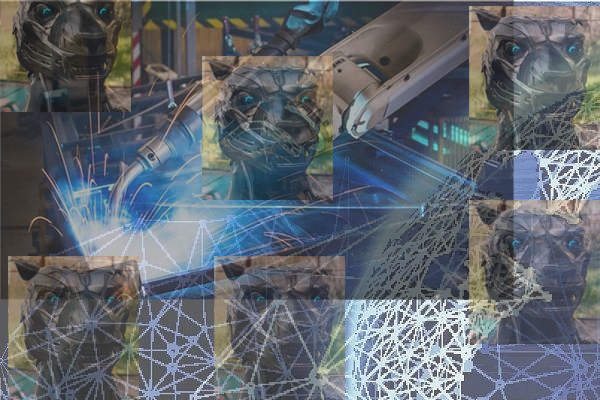
\includegraphics[width=0.76\textwidth]{DistributedAI12180010.jpg}
\caption{}
\label{DistributedAI12180010}
\end{figure}
%%%%%%%%%%%%%%%%%%%%%%%%%%%%%%%%%%%%
%%%%%%%%%%%%%%%%%%%%%%%%%%%%%%%%%%%%%%%%%%%%%%
\section{分布智能}
%%%%%%%%%%%%%%%%%%%%%%%%%%%%%%%%%%%%%%%%%%%%%%
\subsection{分布智能}
\subsubsection{分布智能概述}
%%%%%%%%%%%%%%%%%%%%%%
\subparagraph{分布式问题求解}

分布式问题求解的主要任务是要创建大粒度的协作群体, 使它们能为同一个求解目标而共同工作. 其主要研究内容是如何在多个合作者之间进行任务划分和问题求解. 在分布式问题求解系统中, 数据、知识和控制均分布在各个结点上, 并且没有一个结点能够拥有求解整个问题所需要的足够数据和知识, 因此各结点之间必需通过相互协作才能有效地解决问题.
%%%%%%%%%%%%%%%%%%%%%%
\subparagraph{多Agent系统}
多Agent系统是由多个自主Agent所组成的一种分布式系统. 其主要任务是要创建一群自主的Agent, 并协调它们的智能行为.

多Agent系统与分布式问题求解的主要差别在于, 不同Agent之间的目标可能相同, 但也可能完全不同, 每个Agent都必须具有与其它Agent进行自主协调、协作和协商的能力. 多Agent系统的研究重点包括Agent结构、Agent通信和多Agent合作等.
%%%%%%%%%%%%%%%%%%%%%%%%%%%%%%%%%%%%%%%%%%%%%%
\subsection{Agent的结构}
%%%%%%%%%%%%%%%%%%%%%%
\subparagraph{Agent的基本结构}

Agent结构是指Agent的组成方式. 其基本结构包括反应Agent、慎思Agent及混和Agent的结构.
%%%%%%%%%%%%%%%%%%%%%%
\subparagraph{反应Agent}

    反应Agent是一种不含任何内部状态, 仅是简单地对外界刺激产生响应的Agent. 其结构如图\ref{Agentfansi2020012801}所示, 它采用“感知--动作”工作模式.
%%%%%%%%%%%%%%%%%%%%%%%%%%%%%%%%
\begin{figure}[H]
\centering
  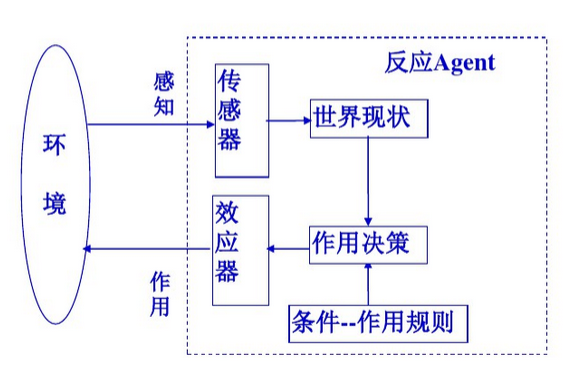
\includegraphics[width=.45\textwidth]{Agentfansi2020012801.PNG}
  \caption{反应Agent的基本结构.}
  \label{Agentfansi2020012801}
\end{figure}

%%%%%%%%%%%%%%%%%%%%%%
\subparagraph{慎思Agent}

慎思Agent的基本结构如图9.3所示. 在该结构中, Agent的基本过程是先通过传感器接收外界环境信息, 并根据内部状态进行信息融合, 然后在知识库支持下制定规划、在目标引导下形成动作序列, 最后由效应器作用于外部环境.
%%%%%%%%%%%%%%%%%%%%%%%%%%%%%%%%
\begin{figure}[H]
\centering
  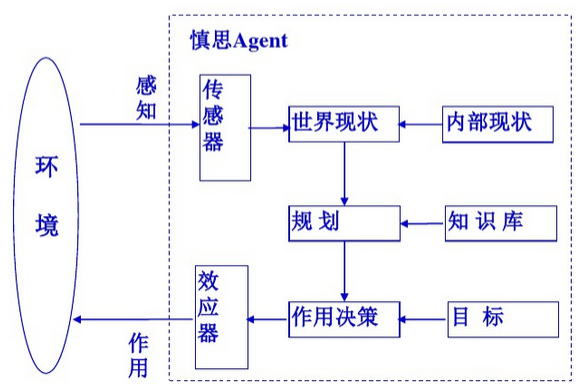
\includegraphics[width=.45\textwidth]{Agentshensi2020012801.PNG}
  \caption{慎思Agent的基本结构.}
  \label{Agentshensi2020012801}
\end{figure}
%%%%%%%%%%%%%%%%%%%%%%
\subparagraph{BDI的概念}
BDI的含义是信念-愿望-意图(Blief-Disire-Intention, 即BDI), 是一种典型的慎思Agent结构.

\begin{itemize}
\item 信念: 是Agent对其环境和自身的认识. 信念不同于知识, 一般认为, 知识是为真的信念. 下面是关于信念的几种不同的解释:

     信念表示尚未完全证实的命题.

     信念表示不一定正确的命题.

     信念表示对已有证据积累的一种函数, 即对命题的相信程度.

\item 愿望: 是Agent希望达到的目标, 这些目标有可能有机会去实现, 但也有可能永远无法实现. 在实际应用中, 一个Agent的初始愿望, 通常是人交给Agent的任务.
\item 意图: 是Agent为达到愿望而计划采取的动作步骤. 意图又可看作是Agent行为的控制器, 它将引导和控制Agent的当前选择和未来活动. 一个Agent的意图有可能会随着环境的变化而改变, 即采取新的动作步骤.
\end{itemize}
%%%%%%%%%%%%%%%%%%%%%%%%%%%%%%%%%%%%%%%%%%%%%%
\subsection{Agent通信}
\subsubsection{Agent通信的基本问题}

    是指多Agent系统中不同Agent之间的信息交换: 其基本问题包括:

通信方式

    Agent通信方式是指不同Agent之间的信息交换方式. 常用的通信方式有消息传送和黑板系统等.

通信语言

    Agent通信语言是指相互交换信息的Agent之间共同遵守的一组语法、语义和语用的定义. 常用的Agent通信语言有知识查询与操纵语言KQML等.

对话管理

    Agent之间的单个信息交换是Agent通信语言需要解决的基本问题, 但Agent之间而往往需要交换一系列信息, 即需要进行对话. 所谓对话是指Agent之间不断进行信息交换的模式, 或者說是Agent之间交换一系列消息的过程.

通信协议
\begin{itemize}
\item Agent通信协议包括Agent通信使用的低层的传输协议和高层的对话协议.
\item 低层的传输协议是指Agent通信中实际使用的低层传输机制, 如TCP、HTTP、FTP、SMTP等.
\item 高层的对话协议是指相互对话的Agent之间的协调协商协议. 常用的描述对话协议的方法有有限状态自动机和Petri网等.
\end{itemize}

知识查询与操纵语言KQML(Knowledge Query and Manipulation Language)是目前国际上最著名的一种Agent通信语言. 它由美国DARPA的知识共享计划KSE研究机构在20世纪90年代开发出来.

KSE开发KQML的主要目的是为了解决基于知识的系统之间, 以及基于知识的系统和常规数据库系统之间的通信问题. 实际上, KSE同时发布的还有一个知识交换格式KIF, 它主要是为了形成KQML的内容部分. 在实际应用中, KQML可基于某种元标记语言(如XML)来实现.
%%%%%%%%%%%%%%%%%%%%%%%%%%%%%%%%%%%%%%%%%%%%%%
\paragraph{通信语言KQML}
%%%%%%%%%%%%%%%%%%%%%%%%%%%%%%%%%%%%%%%%%%%%%%
\subparagraph{KQML语言的结构}

\begin{itemize}
\item 从结构上看, KQML是一种层次结构型语言. 它可分为通信、消息和内容3个层次, 各层的含义如下:
\item 通信层描述的是通信协议和与通信双方有关的一组属性参数, 例如发送者和接受者的身份、与通信有关的标识等.
\item 消息层是KQML语言的核心, 它描述的是与消息有关的言语行为的类型. 其基本功能是确定传送消息所使用的协议和与传送消息有关的语言行为等.
\item 内容层是消息所包含的真正内容, 它可以是任何表示语言、ASCII字符或二进制形式. 对实现来说, KQML并不需要关心消息中内容部分的具体含义.
\end{itemize}

KQML消息: 也称为“行为(performative)原语”或行为表达式, 其基本格式是用一对圆括号括起来的一个表. 表中的第1个元素是消息行为的名称, 后面的元素是一系列参数名及其参数的值.
%%%%%%%%%%%%%%%%%%%%%%%%%%%%%%%%%%%%%%%%%%%%%%
\subparagraph{KQML消息}
可简单地表示为:
\begin{Verbatim}
        (消息行为名称
            : 参数名1   参数值1
            : 参数名2   参数值2
            …)
\end{Verbatim}
其中, 消息行为名称用来指出该消息所引发的语言行为类型, 它由KQML保留的执行原语关键字来描述;参数名及其值用来指出消息的属性、要求和内容等, 它由KQML保留的执行原语参数关键字来描述, 每个参数名都必须以冒号(:)开始, 后接相应的参数值.

KQML语言的最大特点是其消息的参数以关键字为索引, 并且参数的顺序是无关的. 因此, 采用不同语言的异质系统之间能够很方便地分析和处理这些消息.
%%%%%%%%%%%%%%%%%%%%%%%%%%%%%%%%%%%%%%%%%%%%%%
\subparagraph{KQML保留的行为原语参数}
KQML规范中定义了一部分常用的行为原语参数名和与其相关的一些参数值的含义, 这些参数称为保留参数.

这些保留参数是Agent通信中最基本最常用的关键字. 对他们进行统一定义, 可加快异质系统间信息交换和理解的速度. 其参数名及含义如下:
\begin{Verbatim}
    :sender     行为原语的实际发送者
    :receiver   行为原语的实际接收者
    :from    当使用forward转发时, :content中行为原语的最初发送者
    :to    当使用forward转发时, :content中行为原语的最终接收者:
    in-reply-to  对前条消息应答的标记, 其值与前条消息的:reply-with值一致
    :reply-with    对本条消息应答的标记
    :language    :content中内容信息的表示语言的名称
    :ontology    :content中内容信息使用的实体集(如术语定义的集合)名称
    :content    有关行为原语表达内容的信息
\end{Verbatim}

    在上面, content参数表示行为原语的“直接目标”(即它的实际文字意义). content的内容可以用通信双方都能识别的任何语言书写.
%%%%%%%%%%%%%%%%%%%%%%%%%%%%%%%%%%%%%%%%%%%%%%
\subparagraph{KQML保留的行为原语}
KQML中定义的行为原语称为保留的行为原语. 这些行为原语可分为交谈类, 干预和对话机制类, 以及推进与网络类3种类型.

(1) 交谈类原语

    这类原语用来实现Agent间一般信息的交换. 常用的有:
\begin{Verbatim}
    ask-if  :sender想知道:receiver是否认为:content为真.
    tell   :sender向:receiver表明:content在:sender中为真.
    reply  :sender向:receiver传送一个对:receiver的:content的回答.
    advertise    :sender承诺处理嵌入在advertise原语里的所有消息.
\end{Verbatim}
例如, Agent A想发送一个行为表达式到Agent B, 询问bar($x,y$)是否为真, 则其行为原语可表示为:
\begin{Verbatim}
(ask-if
       :sender        A           发送者A
       :receiver      B           接收者B
       :in-reply-to   id0         对前条消息应答的标记
       :reply-with    id1         对本条消息应答的标记
       :language     Prolog       :content中内容使用的语言名称
       :ontology     foo          :content中内容使用的实体集名称
       :content   “bar($x,y$) ”)   表达的内容
\end{Verbatim}

(2) 干预和对话机制类原语

    这类原语用于干预和调整正常的对话过程. 正常的对话过程一般是Agent A发送一条KQML消息给Agent B, 当需要应答或谈话需要继续时, Agent B发送响应消息, 如此循环直到对话结束. 最常用的2条是:
\begin{Verbatim}
    error  :sender不能理解所接收的以:in-reply-to为标识的消息,
            即发送者认为它所接受的前一条消息出错.
    sorry  :sender理解接收到的消息, 消息在语法、语义方面都正确,
            但:sender不能提供任何应答;或者:sender能够提供进一步的应答,
            但由于某种原因它决定不再继续提供. Sorry意味着
                 Agent要终止当前的对话过程.
\end{Verbatim}

(3)网络类原语

    这类原语是为了满足计算机网络通信与服务需要而设立的行为原语. 它们主要由通信服务器Agent使用, 或者其它Agent通过“advertise”原语来使用. 最常用的3条原语是:
\begin{Verbatim}
    register  :sender向:receiver宣告其存在性以及与物理地址有关的符号名.
    forward   :sender希望:receiver传送一条消息给另一个Agent.
    recommend-one:sender请求:receiver推荐一个能够处理:content的Agent.
\end{Verbatim}
%%%%%%%%%%%%%%%%%%%%%%%%%%%%%%%%%%%%%%%%%%%%%%
\subparagraph{KQML通信服务器}
为提高分布式处理的透明性, KQML引入了一个专门用来提供通信服务的特殊的Agent类型, 即被称为通信服务器的facilitator. 它负责各种通信服务, 如: 维护服务名称的注册, 为命名的服务提供消息, 进行基于内容的路由选择等.
%%%%%%%%%%%%%%%%%%%%%%%%%%%%%%%%%%%%%%%%%
\begin{example}
  Agent $A$想知道$x$是否为真, 请求facilitator希望找到一个能够处理ask-if($x$)的Agent;如果在facilitator保存的Agent B有能力处理ask-if($x$), 则facilitator就将Agent B的名字返回给Agent $A$;然后Agent $A$就可以与Agent $B$进行对话, 并得到所需要的答案.
\end{example}

其工作过程如下图所示:

%%%%%%%%%%%%%%%%%%%%%%%%%%%%%%%%%%%%%%%%%%%%%%
\subsection{多Agent合作}
多Agent系统可以看作是一个由一群自主并自私的Agent所构成的一个社会. 在这个社会中, 每个Agent都有自己的利益和目标, 并且它们的利益有可能存在冲突, 目标也有可能不一致.

像人类社会中具有不同利益的人为了实现各自的目标又需要进行合作一样, 多Agent系统也是如此.

    多Agent的合作包括:

    Agent协调: 是指对Agent之间的相互作用和Agent动作之间的内部依赖关系的管理. 它描述的是一种动态行为, 反映的是一种相互作用的性质. 它的两个最基本的成分是: “有限资源的分配”和“中间结果的通信”.

    Agent协作: 协作是指Agent之间相互配合一起工作. 它是非对抗Agent之间保持行为协调的一个特例.

    Agent协商: 协商主要用来消解冲突、共享任务和实现协调, 是多Agent系统实现协调和解决冲突的一种重要方法.


Agent的协调

常用的协调方法有:
\begin{itemize}
\item 基于部分全局规划的协调: 部分全局规划是指将一个Agent组的动作和相互作用进行组合所形成的数据结构.
    所谓规划是部分的, 是指系统不能产生整个问题的规划.
    所谓规划是全局的, 是指Agent通过局部规划的交换与合作, 可以得到一个关于问题求解的全局视图, 进而形成全局规划.
\item 基于联合意图的协调: 意图是Agent为达到愿望而计划采取的动作步骤. 联合意图则是指一组合作Agent对它们所从事的合作活动的整体目标的集体意图.
\item 其典型例子是Agent机器人竞赛中的队内Agent机器人之间的协调问题, 这些Agent既有自己的个体意图, 又有全队的联合意图.
\item 基于社会规范的协调: 基于社会规范的协调是一种以每个Agent都必须遵循的社会规范为基础的协调方法. 所谓规范是一种建立的、期望的行为模式. 社会规范可以对Agent社会中各Agent的行为加以限制, 以过滤掉某些有冲突的意图和行为, 保证其它Agent必须的行为方式, 从而确保Agent自身行为的可能性, 以实现整个Agent社会行为的协调.
\end{itemize}


Agent的协作

    合同网是Agent协作中最著名的一种协作方法, 被广泛应用于各种多Agent系统的协作中. 其思想来源于人们在日常活动中的合同机制. 在合同网系统中, 所有Agent被分为管理者和工作者两种不同角色.

    管理者Agent的主要职责包括:

    (1) 对每一个需要求解的任务建立其任务通知书(Task Announcement), 并将任务通知书发送给有关的工作者Agent;

    (2) 接受并评估来自工作者Agent的投标(Bid);

    (3) 从所有投标中选择最合适的工作者Agent, 并与其签订合同(Contract);

    (4) 监督合同的执行, 并综合结果.

    工作者Agent的主要职责包括:

    (1) 接受相关的任务通知书;

    (2) 评价自己的资格;

    (3) 对感兴趣的子任务返回任务投标;

    (4) 如果投标被接受, 按合同执行分配给自己的子任务;

    (5)  向管理者报告求解结果.

合同网系统的基本工作过程如图\ref{Tu01920121204001}所示:
%%%%%%%%%%%%%%%%%%%%%%%%%%%%%%%%%%%%%%%%%%
\begin{figure}[H]
\centering
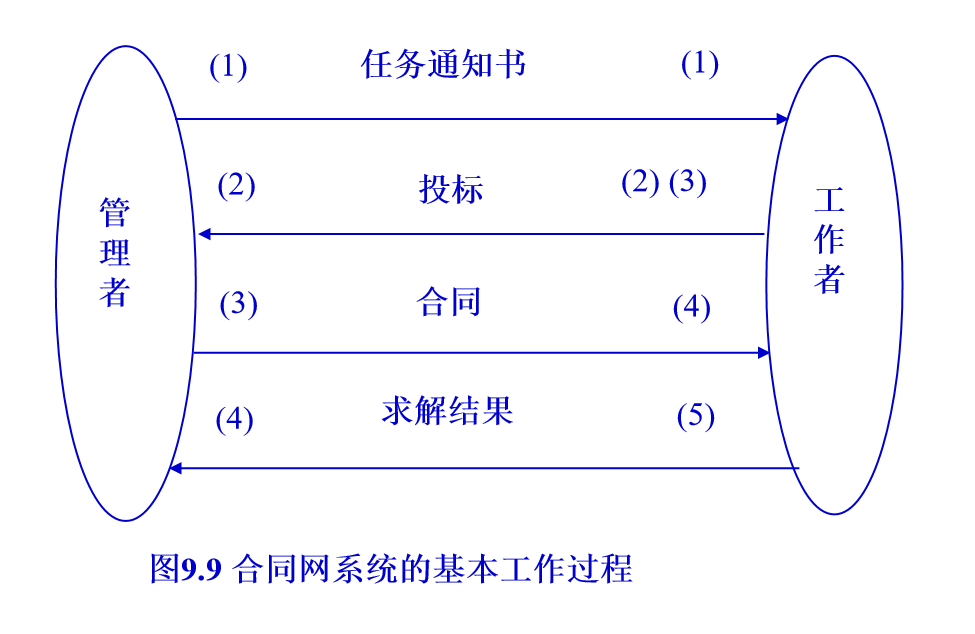
\includegraphics[width=0.6\textwidth]{Tu01920121204001.png}
\caption{语义网络的基本网元}
\label{Tu01920121204001}
\end{figure}
%%%%%%%%%%%%%%%%%%%%%%%%%%%%%%%%%%%%%%%%%%
%%%%%%%%%%%%%%%%%%%%%%%%%%%%%%%%%%%%%%%%%%%%%%
\subsection{Agent的协商}
协商的主要方法包括协商协议、协商策略和协商处理.
%%%%%%%%%%%%%%%%%%%%%%%%%%%%%%%%%%%%%%%%%%%%%%
\subparagraph{协商协议}
    协商协议是用结构化方法描述的多Agent自动协商过程的一个协商行为序列. 它需要详细说明初始化一个协商循环和响应消息的各种可能情况. 最简单的协商协议是按照
\begin{center}
  <协商原语><协商内容>
\end{center}
这种形式定义的一个可能的协商行为序列.
%%%%%%%%%%%%%%%%%%%%%%%%%%%%%%%%%%%%%%%%%%%%%%
\subparagraph{协商策略}
协商策略是模型化Agent内部协商推理的控制策略, 亦是实现协商决策的元级知识, 在协商过程中起着重要的作用. 协商策略主要用于Agent决策及选择协商协议和通信消息.
%%%%%%%%%%%%%%%%%%%%%%%%%%%%%%%%%%%%%%%%%%%%%%
\subparagraph{协商处理}
协商处理包括协商算法和系统分析两个方面. 其中, 协商算法用于描述Agent在协商过程中的行为, 如通信、决策、规划和知识库操作等;系统分析用于分析和评价Agent协商的行为和性能, 回答协商过程中的问题求解质量、算法效率和公平性等问题.

\href{https://www.sciencedirect.com/journal/decision-support-systems}{决策支持系统杂志}.
%%%%%%%%%%%%%%%%%%%%%%%%%%%%%%%%%%%%%%%%%%%%%%
\subparagraph{多Agent应用示例}
多Agent系统的应用非常广泛, 诸如智能信息检索、分布式网络管理、电子商务、协同工作和智能网络教学系统等. 以智能网络教学系统为例:
%%%%%%%%%%%%%%%%%%%%%%%%%%%%%%%%%%%%%
\begin{example}
学生模型数据库是学生知识结构的反映. 数据库Agent负责学生模型数据库、教学Agent群和界面Agent之间交互的管理. 教学策略Agent群中的每个Agent都相当于一个教育家. 教学过程管理Agent的主要功能是监视教学过程, 并向教学Agent提供教学参考意见. 教学Agent群是整个智能教学系统的核心, 其中的每个教学Agent都相当于一个教师. 界面Agent构成了系统的交互模型, 他主要负责与学生或教师的交互.
\end{example}
%%%%%%%%%%%%%%%%%%%%%%%%%%%%%%%%%%%%%%%%%%%%%%
\subsection{移动Agent}
移动Agent( MA)是一种可以从网络上一个结点自主地移动到另一个结点, 实现分布式问题处理的特殊的Agent. 它由移动Agent和移动Agent环境两大部分所组成.
%%%%%%%%%%%%%%%%%%%%%%%%%%%%%%%%%%%%%%%%%%%%%%
\section{作 业}
%%%%%%%%%%%%%%%%%%%%%%%%%%%%%%%%%%%%%%%%%%%%%%%%
\begin{think}
Agent在结构上有什么特点?它是如何按照结构进行分类的?
\end{think}
%%%%%%%%%%%%%%%%%%%%%%%%%%%%%%%%%%%%%%%%%%%%%%%%
\begin{think}
什么是协调、协作、协商?它们之间有什么联系和区别?
\end{think}
